\documentclass[11pt,a4paper]{article}
\usepackage[margin=2.2cm]{geometry}
\usepackage{amsmath,amssymb}
\usepackage{siunitx}
\usepackage{booktabs}
\usepackage{xcolor}
\usepackage{microtype}
\usepackage{enumitem}
\usepackage{tcolorbox}
\usepackage{graphicx}
\definecolor{ink}{HTML}{14231B}\definecolor{accent}{HTML}{0F3D2A}
\tcbuselibrary{skins}
\newtcolorbox{key}{colback=accent!6,colframe=accent,boxrule=0.6pt,arc=2pt,left=6pt,right=6pt,top=4pt,bottom=4pt}
\sisetup{per-mode=symbol,group-separator={\,}}
\setlength{\parindent}{0pt}\setlength{\parskip}{6pt}
\renewcommand{\arraystretch}{1.25}

\title{\textbf{Slide 4: high-pass filter}\\\large Cut the plant noise below the AE band}
\author{ADS7057 test board v3 \quad ---\quad study notes}\date{}
\begin{document}\maketitle\vspace{-1.2em}
\section{Why the board needs a high-pass}
Eight baseline records, taken with no event, show where the noise sits. Below \SI{100}{kHz} it is \SI{11.5}{} to \SI{26.8}{mV} rms. Inside the AE band (100 to \SI{500}{kHz}) five records show only \SI{3.7}{} to \SI{4.6}{mV} rms. Events are \SI{234}{} to \SI{275}{kHz}. A high-pass just under the band removes the large low-frequency noise before the gain stage amplifies it by 4.9.

\begin{center}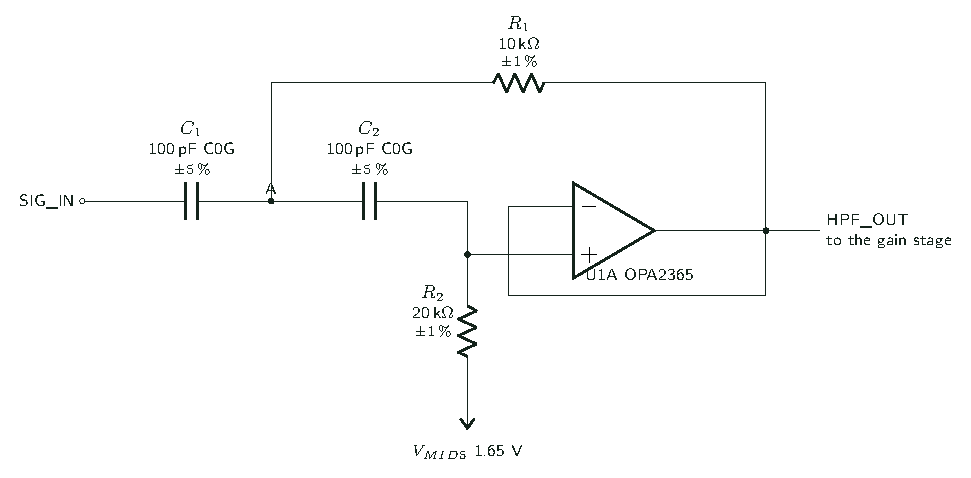
\includegraphics[width=0.98\textwidth]{s04_circuit.pdf}\end{center}

\section{Derivation from the node equations}
U1A is a voltage follower, so the output equals the voltage at its $+$ input: $V_o=V_B$. The current into each node must sum to zero (all voltages are deviations from VMID5, so R2 goes to 0).

\textbf{Node B} (the $+$ input draws no current):
\[
(V_B-V_A)\,sC_2+\frac{V_B}{R_2}=0
\;\Rightarrow\;
V_A=V_B\Big(1+\frac{1}{sR_2C_2}\Big).
\]
\textbf{Node A:}
\[
(V_A-V_{in})\,sC_1+(V_A-V_B)\,sC_2+\frac{V_A-V_o}{R_1}=0,\qquad V_o=V_B .
\]
Substitute $V_A$ and collect $V_B$:
\[
sC_1V_{in}=V_B\Big[sC_1+\frac{C_1+C_2}{R_2C_2}+\frac{1}{sR_1R_2C_2}\Big].
\]
Divide by $sC_1$:
\[
\boxed{\;H(s)=\frac{V_B}{V_{in}}=\frac{s^2}{s^2+s\,\dfrac{C_1+C_2}{R_2C_1C_2}+\dfrac{1}{R_1R_2C_1C_2}}\;}
\]
Compare with the standard second-order form $s^2/(s^2+s\,\omega_0/Q+\omega_0^2)$:
\[
\omega_0=\frac{1}{\sqrt{R_1R_2C_1C_2}},\qquad
\frac{\omega_0}{Q}=\frac{C_1+C_2}{R_2C_1C_2}.
\]
With $C_1=C_2=C$:
\[
f_0=\frac{1}{2\pi C\sqrt{R_1R_2}}=\frac{1}{2\pi\cdot100\,\text{pF}\cdot\sqrt{10\,\text{k}\Omega\cdot20\,\text{k}\Omega}}=\SI{112.5}{kHz},
\qquad
Q=\frac12\sqrt{\frac{R_2}{R_1}}=\frac12\sqrt2=0.707 .
\]
\begin{key}
$Q=0.707$ is the Butterworth value: the flattest magnitude with no peak. The rejection below the corner is $-40$\,dB per decade, because the numerator is $s^2$. At \SI{10}{kHz}: $(10/112.5)^2\approx0.008=\SI{-42}{dB}$.
\end{key}

\begin{center}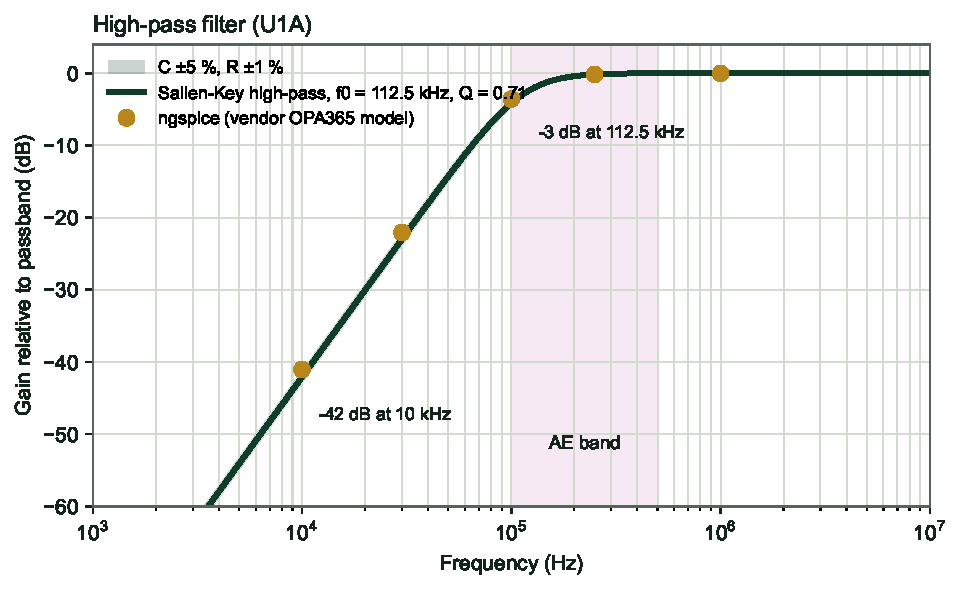
\includegraphics[width=0.78\textwidth]{s04_graph.pdf}\end{center}

\section{Why these values}
\begin{itemize}[nosep]
\item \textbf{Corner at 112.5\,kHz}: just under the AE band. A higher corner would also cut the events. The loss at \SI{250}{kHz} is only \SI{0.17}{dB}.
\item \textbf{$C_1=C_2$}: then $Q$ depends only on the resistor ratio. Equal C0G capacitors in one value keep the BOM short.
\item \textbf{$R_2$ to VMID5, not ground}: the stage rests at \SI{1.65}{V}, so the single supply never clips the negative half.
\item \textbf{OPA2365, GBW \SI{50}{MHz}}: the follower stays accurate far above the corner. Finite gain changes $H$ by less than 0.01\,dB at \SI{250}{kHz}.
\end{itemize}

\section{Tolerances}
Capacitors are C0G $\pm5\,\%$ (C14858), resistors $\pm1\,\%$ (C25804, C4184). Over all 16 corner combinations of $C_1$, $C_2$, $R_1$, $R_2$:
\[
f_0=\SI{106.1}{} \text{ to } \SI{119.7}{kHz},\qquad Q=0.699 \text{ to } 0.714 .
\]
The corner moves about $\pm6\,\%$. $Q$ stays within 1\,\% of 0.707, so the response keeps its shape. The grey band in the plot is a random sample of these tolerances.
\end{document}
